\chapter{Statistical distribution functions of random variables}\label{Section_3.3}
In this appendix, statistical distribution functions of random variables are addressed.

\section{Generic description of the application of distribution functions}\label{Section_3.3.1}
The following three types of functions can be used to describe the statistical properties of random variables: 
\begin{enumerate}
\item Cumulative distribution function (CDF);
\item Inverse cumulative distribution function (inverse CDF);
\item Probability density function (PDF).
\end{enumerate}

The CDF, $F(x)$, provides the probability of non-exceedance, p, of each potential realisation, $x$, of random variable $X$. The inverse CDF, $F^{-1}(p)$, provides the realisation $x$ that has a probability of non-exceedance $p$. The relation between the CDF and the inverse CDF is thus as follows: 
\begin{equation}
F\left(x\right)=p\Leftrightarrow x=F^{-1} \left(p\right) \label{3.1)}
\end{equation}

The PDF, $f(x)$, is the derivative of the CDF:
\begin{equation}
F\left(x\right)=\int _{-\infty }^{x}f\left(\tau \right)d \tau \Leftrightarrow f\left(x\right)=\frac{dF}{dx} (x) \label{3.2)}
\end{equation}

The PDF provides the probability density for any given value of $x$. The probability density is the probability per unit value. For the normal distribution function, the pdf is the ''famous'' bell-shaped curve. As an example, \Fref{fig:Figure_3.2} shows the CDF, inverse CDF and PDF of the standard normal distribution function. 

\begin{figure}[H]\centering
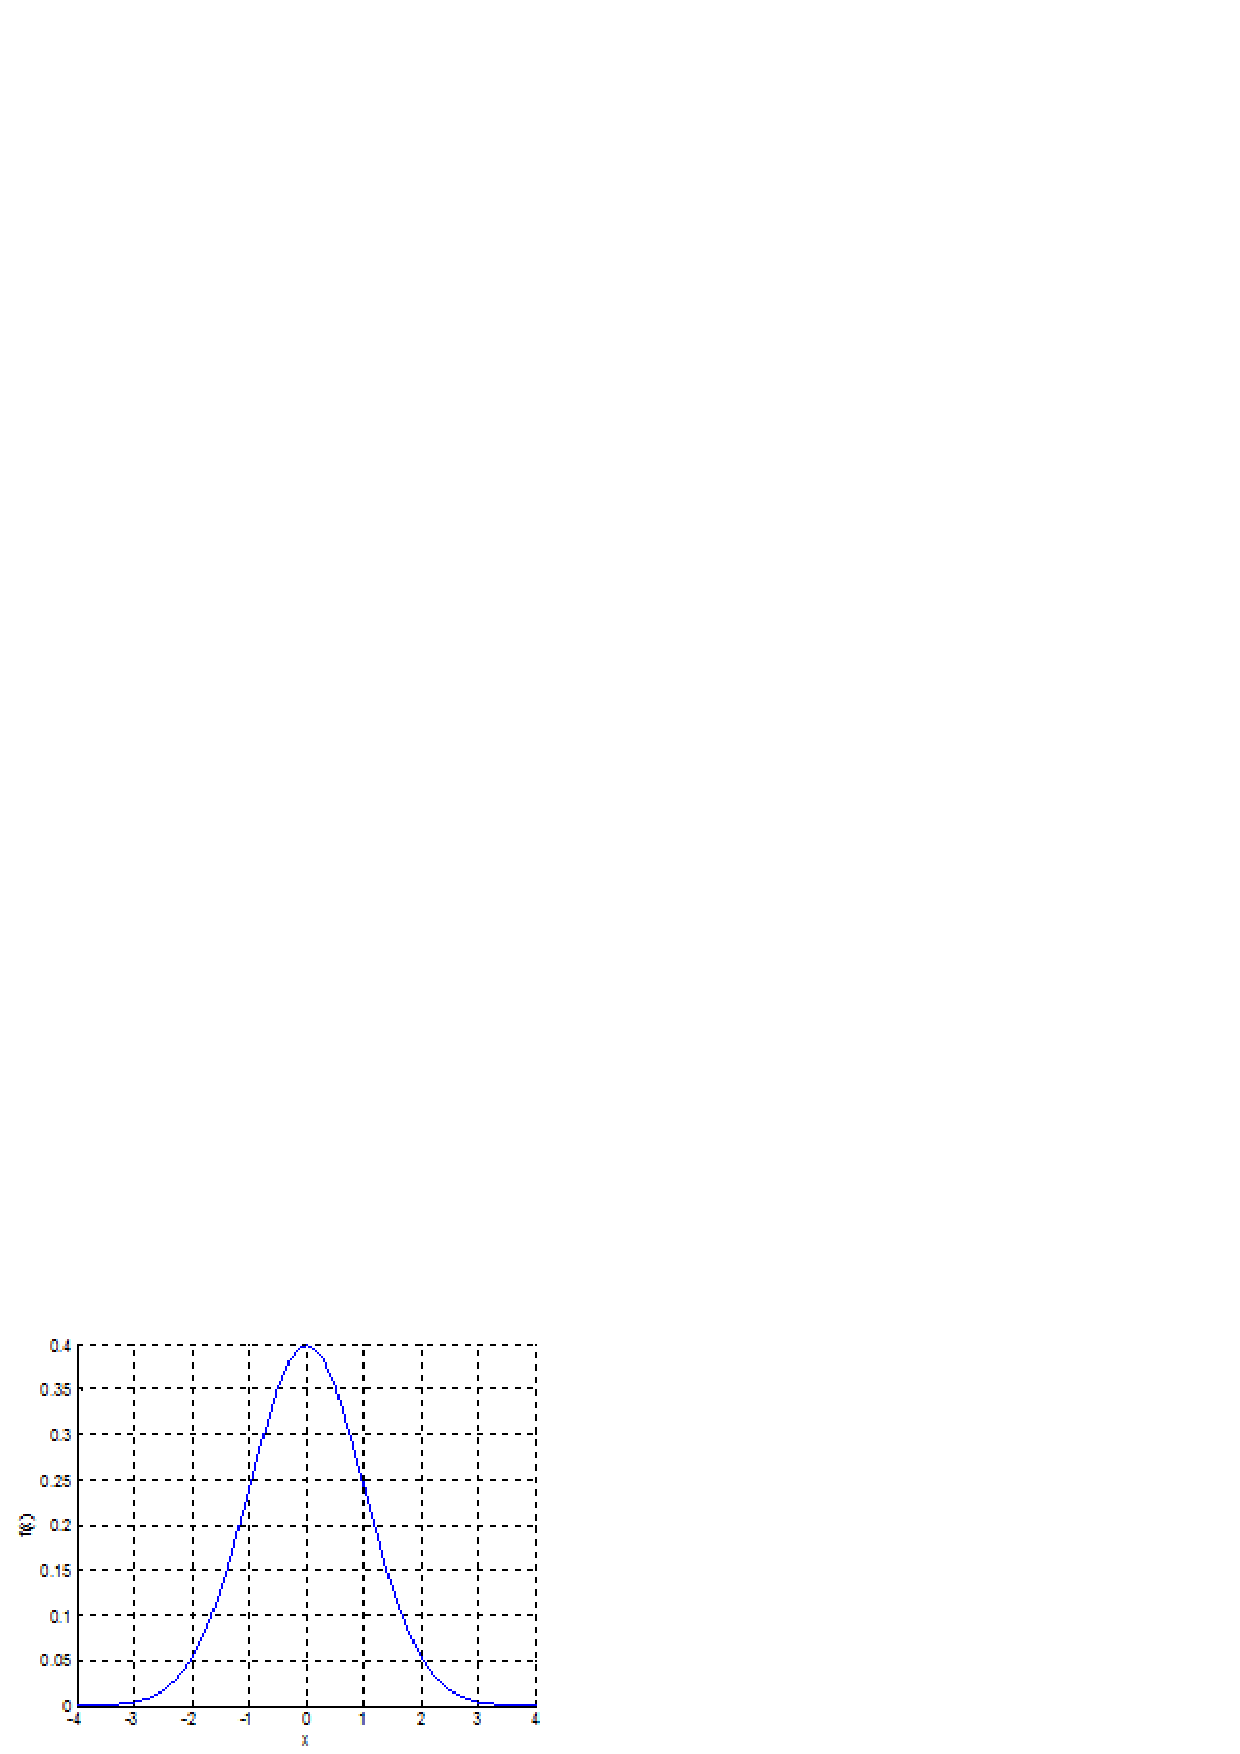
\includegraphics[width=0.55\columnwidth]{funcdesign_chapters/figloadmodels/image51.png}
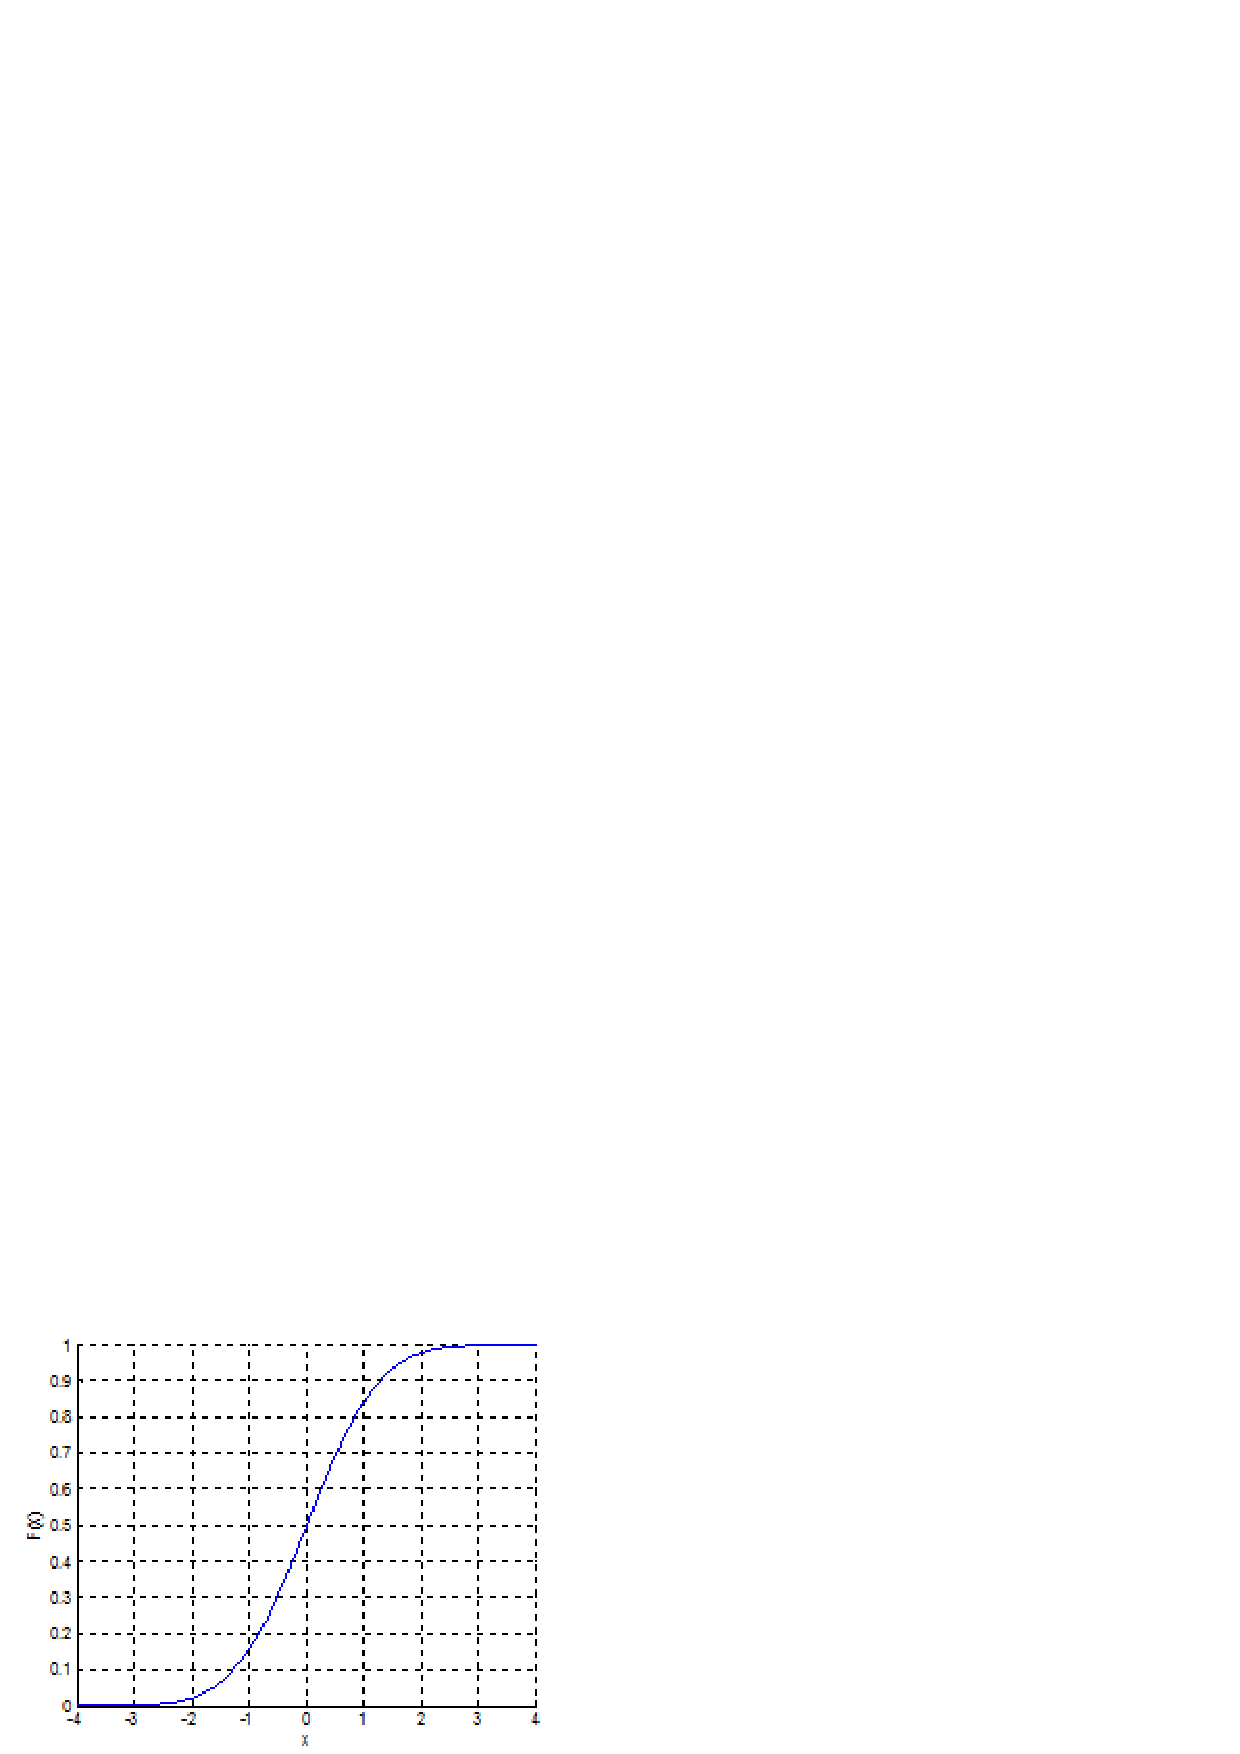
\includegraphics[width=0.55\columnwidth]{funcdesign_chapters/figloadmodels/image52.png}
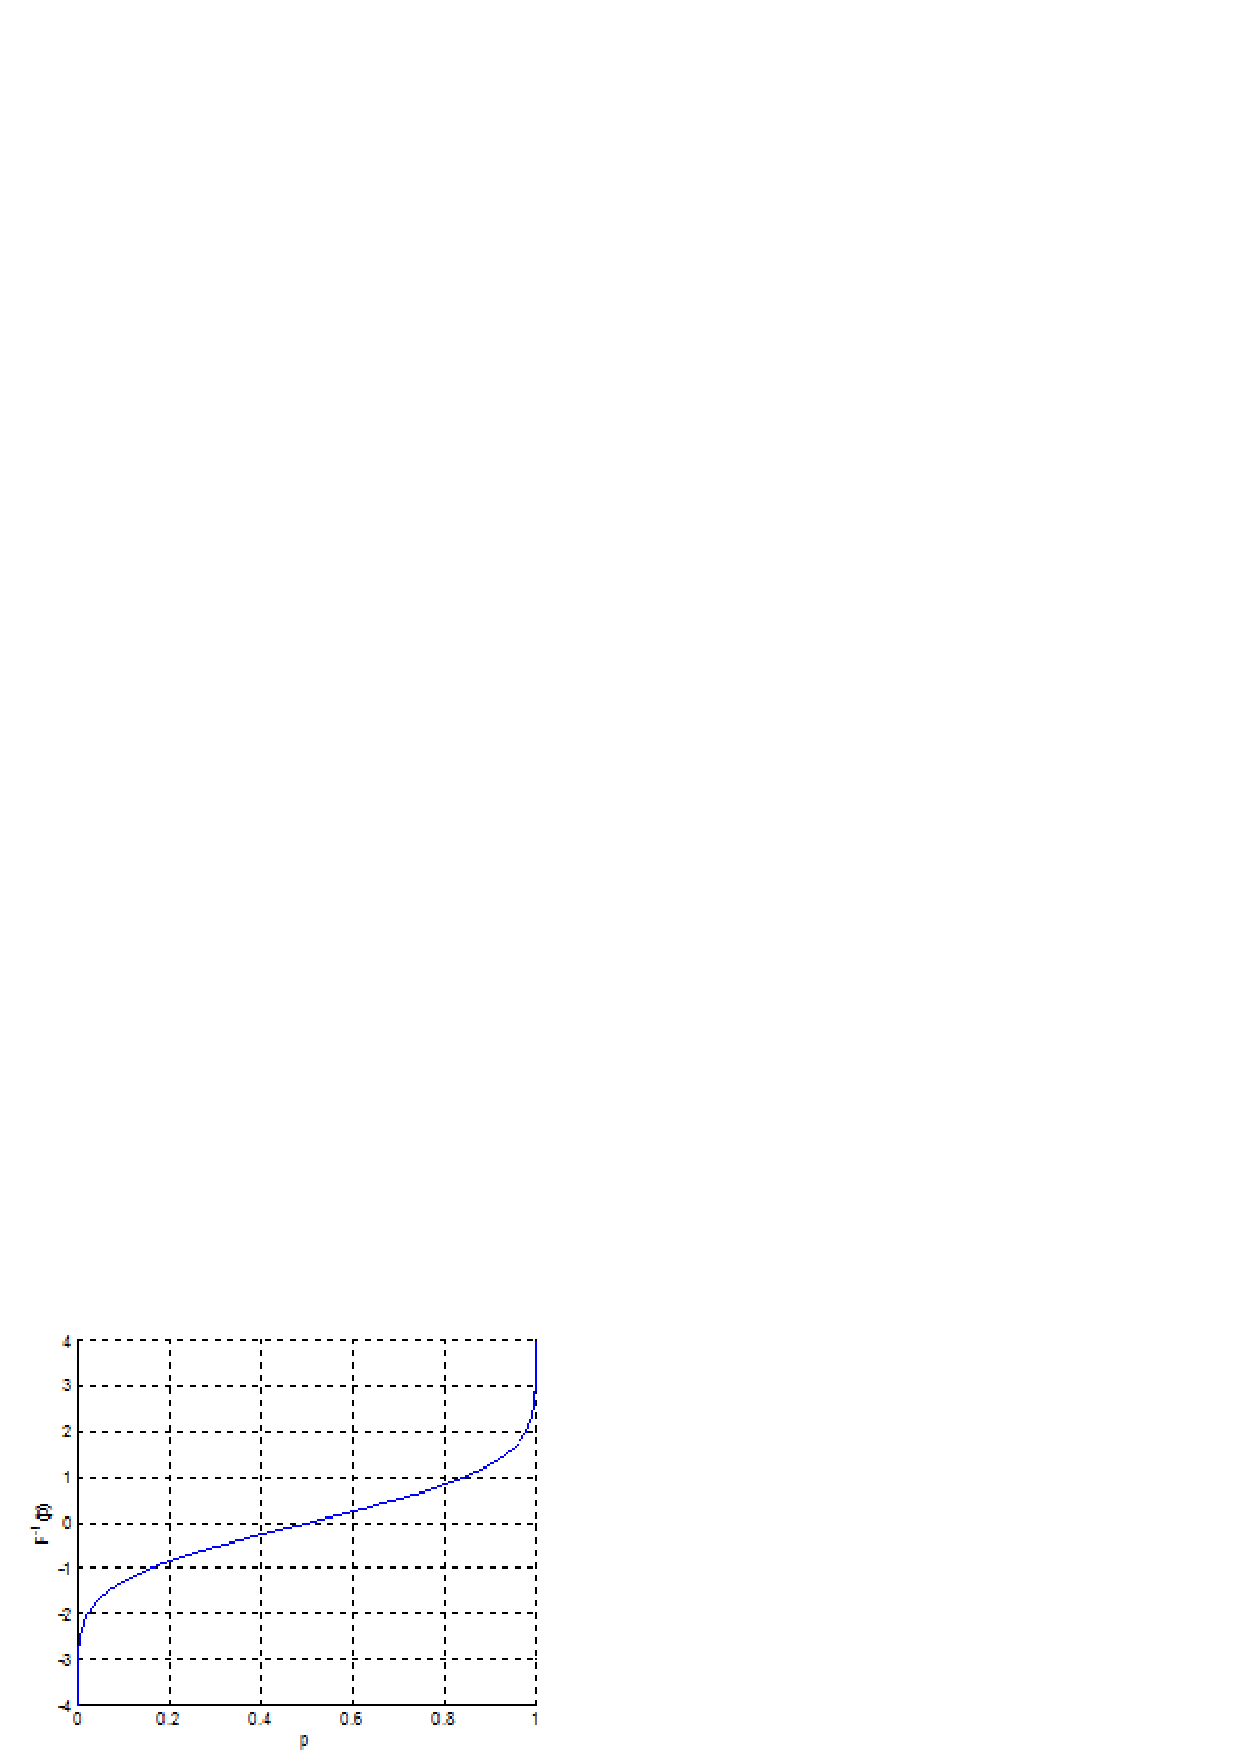
\includegraphics[width=0.55\columnwidth]{funcdesign_chapters/figloadmodels/image53.png}
\caption{PDF (top), CDF (middle) and inverse CDF (bottom) of the standard normal distribution function.}\label{fig:Figure_3.2}
\end{figure}

The CDF, $F(x)$, has the flowing properties:
\begin{enumerate}
\item $F(x)$ is non-decreasing;
\item $\lim_{x\rightarrow -\infty}F(x)=0$;
\item $\lim_{x\rightarrow \infty}F(x)=1$.
\end{enumerate}

Property 1 can be easily proven: if $x_1<x_2$, then $P[X\leq x_1] \leq P[X\leq x_2]$ and thus $F(x_1) \leq F(x_2)$. For a formal proof of properties 2 and 3, the reader is referred to \cite{GrimmettStirzaker1983}. But even without a proof it is intuitively clear that a realization from a probability function will be lower than $\infty$ and higher than -$\infty$.

Since $F(x)$ is non-decreasing, the inverse CDF, $F^{-1}(p)$, is also a non-decreasing function. In probabilistic computations, mainly the inverse CDF, $F^{-1}(x)$, of a variable $X$ is applied, as schematically depicted in \Fref{fig:Figure_3.3}. The library of distribution functions therefore mostly consists of inverse CDF's. The procedure of \Fref{fig:Figure_3.3} is explained below.

\begin{figure}[H]\centering
\includegraphics*[width=3.95in, height=2.59in, keepaspectratio=false]{funcdesign_chapters/figloadmodels/image54.png}
\caption{Procedure for determining a load variable associated with a randomly selected standard normally distributed variable ($u$-value), for the case of uncorrelated variables.}\label{fig:Figure_3.3}
\end{figure}

As described in section \Aref{Section_2.3}, random variables are represented by standardised $U$-variables in the probabilistic computations in the \probLib, and the function $Z(U)$ is explored to derive an estimate of the failure probability. In order to evaluate function $Z(U)$, the realisations of the $U$-variables are first translated to the corresponding realisations of the $X$-variables and subsequently the $Z$-value is determined. Assume for the sake of simplicity that the $X$-variables are mutually independent (correlations will be dealt with in \Aref{Section_3.4}). As explained in \Aref{Section_2.2.3}, the transformation from a realization, $u$, of variable $U$, to realization $x$, of variable $X$, is done in such a away that the (non-)exceedance probabilities of $u$ and $x$ are equal. This transformation, as depicted in \Fref{fig:Figure_3.3}, can be formulated as follows:
\begin{equation}
\Phi \left(u\right)=F\left(x\right)\; \quad \Rightarrow \; \quad x=F^{-1} \left(\Phi \left(u\right)\right) \label{ZEqnNum694082}
\end{equation}
where:

\begin{tabular}{lll}
$\Phi$ &=& standard normal distribution function\\
$F$ &=& CDF of variable $X$\\
$F^{-1}$ &=& inverse CDF of $X$\\
$x$ &=& realisation of $X$\\
$u$ &=& realisation of $U$\\
\end{tabular}

This procedure automatically guarantees that variable $x$ is a realization from distribution function $F(x)$ and therefore correctly represents the statistical properties of variable $X$. This is demonstrated below.

First it needs to be shown that the value $p = \Phi(u)$ is a realization from a standard uniform distribution function. The standard uniform distribution function is the CDF in which each value in the range $[0,1]$ has equal probability density. The CDF of this function is as follows (see also \Fref{fig:Figure_3.4}):
\begin{equation}
F\left(x\right)\; =\left\{\begin{array}{l} {0\quad ;x\le 0\quad } \\ {\; x\quad ;0<x<1} \\ {1\quad ;x\ge 1\quad } \end{array}\right. \quad \label{ZEqnNum892201}
\end{equation}

Consider a realization, $u^*$, of the standard normal distribution function with a probability of non-exceedance equal to $p^* = \Phi(u^*)$. By definition this means that the probability that a random sample $u$ from the standard normal distribution function does not exceed $u^*$ is equal to $p^*$. In formula:
\begin{equation}
P\left[u\le u^*\right]=p^* \label{ZEqnNum312921}
\end{equation}

Since $\Phi$ is a CDF, it is a non-decreasing function. Therefore it follows from equation \eqref{ZEqnNum312921} that:
\begin{equation}
P\left[\Phi \left(u\right)\le \Phi \left(u^*\right)\right]=p^*\label{3.6)}
\end{equation}

And since by definition $p^*= \Phi(u^*)$, this simplifies to:
\begin{equation}
P\left[\Phi \left(u\right)\le p^*\right]=p^* \label{3.7)}
\end{equation}

So the probability that $\Phi(u)$ does not exceed a given value $p^*$ ($0\leq p^* \leq 1$) is equal to $p^*$. This shows that $\Phi(u)$ is a realization from a standard uniform distribution function, as described by equation \eqref{ZEqnNum892201} and depicted in \Fref{fig:Figure_3.4}.

\begin{figure}[H]\centering
\includegraphics*[width=4.28in, height=3.21in, keepaspectratio=false]{funcdesign_chapters/figloadmodels/image55.png}
\caption{Standard uniform distribution function (CDF).}\label{fig:Figure_3.4}
\end{figure}

It has been demonstrated that the value $p$ in \Fref{fig:Figure_3.3} is a realization from the standard uniform distribution function. The next step is to show that the value $x = F^{-1}(p)$ in \Fref{fig:Figure_3.3} is a realization from distribution function $F(x)$. For this purpose, consider a value $x^*$ with probability of non-exceedance $p^*$. This means: $F(x^*) = p^*$ and $x^* = F^{-1}(p^*)$. The value $p$ in \Fref{fig:Figure_3.3} is taken from a standard uniform distribution function (as proven above), which means:
\begin{equation}
P\left[p\le p^*\right]=p^*\label{ZEqnNum788001}
\end{equation}

Since $F$ is an inverse CDF, it is a non-decreasing function and therefore it follows from equation \eqref{ZEqnNum788001} that:
\begin{equation}
P\left[F^{-1} \left(p\right)\le F^{-1} \left(p^*\right)\right]=p^*\label{ZEqnNum178723} 
\end{equation}

By definition $x^* = F^{-1}(p^*)$ and $x = F^{-1}(p)$, which means equation \eqref{ZEqnNum178723} simplifies to:
\begin{equation}
P\left[x\le x^*\right]=p^*\label{3.10)} 
\end{equation}

Since $p^*= F(x)$, this means: 
\begin{equation} 
P\left[x\le x^*\right]=F\left(x^*\right)\label{3.11)} 
\end{equation}

This shows that value $x$ in \Fref{fig:Figure_3.3} is a realization from distribution function $F(x)$. 

\Note{the \probLib works with standard normalized $U$-variables. The limit state function $Z(U)$ is explored to derive an estimate of the failure probability. In order to evaluate function $Z(U)$, the realisations of the $U$-variables are first translated to the corresponding realisations of the $X$-variables to be able to determine the $Z$-value. In this transformation, the inverse CDF of variable $X$ is applied, to provide variable $X$ with the correct statistical properties.}

\Note{\Aref{app:distributionfunctions} presents distribution functions available in the \probLib.The library contains the ''inverse cumulative distribution functions'' which means the input consists of a probability, $p$, of non-exceedance and the output consist of the associated realization, $x$, of the variable that is described with this distribution function.} 

%Besides $p$, the input of the inverse CDF's also consists of a set of parameter values $\theta = (\theta_1, \dots ,\theta_n)$. These parameter values quantify the relation between $p$ and $x$. Note that the value of $n$ can be different for different distribution functions, as shown in the second column of \Tref{Table_3.1}. Each distribution function as mentioned in \Tref{Table_3.1} has a fixed number, $n$, of parameters but the values of these parameters will be different for different variables. So, for instance, it is possible to describe both river discharge and sea water level with the lognormal distribution, but the values of the two parameters of this distribution function for river discharge will be different from the values that are used for sea water level. In other words: the same module can be used to describe probabilities of different random variables and differences between the variables are characterized by differences in parameter values. 

\section{Probability distribution functions}\label{app:distributionfunctions}

\subsection{Deterministic distribution\label{sec:deterministicdistribution}}

A deterministic random variable takes a certain value, let's say value $x_0$, with probability $1$. The cumulative distribution function of such variable is given as follows:
\begin{align}
F(x) = \left\{\begin{array}{l} {1\mbox{ for }x\geq x_0} \\ {0 \mbox{ for }x<x_0} \end{array}\right.
\end{align}

\subsection{Uniform distribution\label{sec:uniformdistribution}}

The probability density function for the uniform distribution is given by:
\begin{align}
f\left(x\right)=\left\{\begin{array}{l} {\frac{1}{b-a}\mbox{ for }a\le x\le b} \\ {0\mbox{ for }x<a\mbox{ or }x>b} \end{array}\right. \label{4.72)} 
\end{align}

The corresponding cumulative distribution function is given by: 
\begin{align}
F\left(x\right)=\left\{\begin{array}{l} {0\mbox{ for }x<a} \\ {\frac{x-a}{b-a} \mbox{ for }a\le x<b} \\ {1\mbox{ for }x\ge b} \end{array}\right. \label{4.73)} 
\end{align}

The inverse of the uniform distribution is given by:
\begin{align}
F^{-1} \left(p\right)=a+p\left(b-a\right),    p\in \left(0,1\right) \label{4.74)} 
\end{align}

The inverse, $F^{-1}$, gives the value of $x$ associated for a given value of the probability of non-exceedance, $p$. 

The distribution parameters a and $B$ indicate the range over which the probability density function is non-zero, with a indicating the starting point and $B$ indicating the ending point. \Fref{fig:A.1} and \Fref{fig:A.2} show the uniform probability density and cumulative probability distribution, respectively, as a function of a and b. 

\begin{figure}[H]\centering
\includegraphics*[width=3.04in, height=2.33in, keepaspectratio=false]{funcdesign_chapters/figappdistributionfunctions/image30}
\caption{Uniform probability density function, with parameters $a$ and $B$ indicated}\label{fig:A.1}
\end{figure}

\begin{figure}[H]\centering
\includegraphics*[width=2.85in, height=2.34in, keepaspectratio=false]{funcdesign_chapters/figappdistributionfunctions/image31}
\caption{Uniform cumulative distribution function, with parameters $a$ and $B$ indicated}\label{fig:A.2}
\end{figure}


\subsection{Normal distribution\label{sec:normaldistribution}}
The probability density function for the normal distribution is given by:
\begin{align}
f\left(x\right)=\frac{1}{\sqrt{2\pi \sigma ^{2} } } \exp \left[-\frac{\left(x-\mu \right)^{2} }{2\sigma ^{2} } \right] \label{4.75)} 
\end{align}

The corresponding cumulative distribution function is given by: 
\begin{align}
F\left(x\right)=\frac{1}{2} \left[1+\mbox{erf}\left(\frac{x-u}{\sqrt{2\sigma ^{2} } } \right)\right] \label{4.76)} 
\end{align}

where erf refers to the error function, which is expressed as follows:
\begin{align}
\mbox{erf}\left(x\right)=\frac{2}{\sqrt{\pi } } \int _{0}^{x}e^{-t^{2} } dt \label{4.77)} 
\end{align}

The standard normal distribution, denoted by $\Phi$, is the special case of the normal distribution for which the mean is equal to zero and the standard deviation is equal to one. For the special case of the standard normal distribution, the inverse is given as follows: 
\begin{align}
\Phi ^{-1} \left(p\right)=\sqrt{2} \cdot \textrm{erf}^{-1} \left(2p-1\right),   p\in \left(0,1\right) \label{ZEqnNum712080} 
\end{align}

For the general case of a normal distribution with mean $\mu $ and standard deviation $\sigma $, the inverse is given as follows:
\begin{align}
F^{-1} \left(p;\mu ,\sigma ^{2} \right)=\mu +\sigma \cdot \Phi ^{-1} \left(p\right),   p\in \left(0,1\right) \label{ZEqnNum182159} 
\end{align}

\Note{there is no explicit form for the normal distribution or inverse normal distribution;
therefore, these functions need to be approximated numerically. The method implemented in the \probLib is described in \Aref{appConversions}.}

\Fref{fig:A.3} shows the probability density of the normal distribution, with the parameters $\mu $ and $\sigma $ indicated. \Fref{fig:A.4} shows the variation in the density function for different choices of $\mu $ and $\sigma $.

\begin{figure}[H]\centering
\includegraphics*[width=2.76in, height=2.33in, keepaspectratio=false]{funcdesign_chapters/figappdistributionfunctions/image32}
\caption{Normal probability density function, with parameters $\mu $ and $\sigma $ indicated}\label{fig:A.3}
\end{figure}

\begin{figure}[H]\centering
\includegraphics*[width=4.10in, height=3.22in, keepaspectratio=false]{funcdesign_chapters/figappdistributionfunctions/image33}
\caption{Illustration of the effect of parameters $\mu $ and $\sigma $}\label{fig:A.4}
\end{figure}


\subsection{(Shifted) Lognormal distribution\label{sec:lognormaldistribution}}
The lognormal distribution is a probability distribution of a random variable whose logarithm is normally distributed. That is, if $x$ is a random variable with a lognormal distribution, then $Y$ = log($x$) is normally distributed, and similarly if $Y$ is a random variable with a normal distribution, exp(y) is lognormally distributed.

The lognormal density function is given as follows:
\begin{align}
f\left(x;\mu ,\sigma ,\varepsilon \right)=\frac{1}{\left(x-\varepsilon \right)\sqrt{2\pi \sigma ^{2} } } \exp \left[-\frac{\left(\ln \left(x-\varepsilon \right)-\mu \right)^{2} }{2\sigma ^{2} } \right],    x>0 \label{4.80)} 
\end{align}
%\todo{ddierman3:what is the added value of $\varepsilon$? It seems $\mu$ suffices for the shift}

The corresponding cumulative distribution function is given by: 
\begin{align}
F\left(x\right)=\Phi \left(\frac{\ln \left(x-\varepsilon \right)-\mu }{\sigma } \right) \label{4.81)} 
\end{align}

where $\Phi$ is the standard normal distribution function described in \Aref{sec:normaldistribution}. 

The parameters of the lognormal distribution, $\mu $ and $\sigma $, are the mean and standard deviation of the associated normally distributed variable. That is, if $x$ is lognormally distributed, and $Y$ = log($x$) is normally distributed, the lognormal parameters $\mu $ and $\sigma $ are the mean and standard deviation of y. The parameter $\varepsilon $ is the shift parameter and serves to horizontally translate the distribution. \Fref{fig:A.5} shows the effect of different choices of the parameters.

\begin{figure}[H]\centering
\includegraphics*[width=4.10in, height=3.22in, keepaspectratio=false]{funcdesign_chapters/figappdistributionfunctions/image34}
\caption{Illustration of the effect of parameters $\mu $, $\sigma $, and $\varepsilon $ on the lognormal density function}\label{fig:A.5}
\end{figure}

To get the inverse distribution, the following steps are taken. The first step is, for a given probability p, the inverse standard normal variable is computed by numerically solving equation \eqref{ZEqnNum712080}. The associated normal variable with mean $\mu $ and standard deviation $\sigma $ is then computed analytically using equation \eqref{ZEqnNum182159}. The relationship between the normal and lognormal distributions is then exploited:
\begin{align}
F^{-1} \left(p;\mu ,\sigma \right)=\exp \left[\mu +\sigma \cdot \Phi ^{-1} \left(p\right)\right]+\varepsilon ,    p\in \left(0,1\right)\label{4.82)} 
\end{align}

\subsection{(Shifted) Exponential distribution\label{sec:exponentialdistribution}}
The density function for the shifted exponential distribution is given as follows:
\begin{align}
f\left(x;\lambda ,\varepsilon \right)=\left\{\begin{array}{l} {\lambda \exp \left[-\lambda \cdot \left(x-\varepsilon \right)\right],    x>\varepsilon } \\ {0,                                          x<\varepsilon } \end{array}\right. \label{4.83)} 
\end{align}

The corresponding cumulative distribution function is given by: 
\begin{align}
F\left(x;\lambda ,\varepsilon \right)=\left\{\begin{array}{l} {1-\exp \left[-\lambda \cdot \left(x-\varepsilon \right)\right],    x\ge \varepsilon } \\ {0\qquad\qquad\qquad\qquad\qquad ,x<\varepsilon } \end{array}\right. \label{4.84)} 
\end{align}

The inverse distribution can be analytically computed from the distribution function:

 
\begin{align}
F^{-1} \left(p;\lambda ,\varepsilon \right)=\varepsilon -\frac{\ln \left(1-p\right)}{\lambda } . \label{4.85)} 
\end{align}

The parameter of the exponential distribution, $\lambda $, is referred to as a rate parameter, and determines how quickly the density function goes to zero. The parameter $\varepsilon $ is the shift parameter and serves to horizontally translate the density. \Fref{fig:A.5} shows the effect of different choices of the parameters.

\begin{figure}[H]\centering
\includegraphics*[width=4.17in, height=3.27in, keepaspectratio=false]{funcdesign_chapters/figappdistributionfunctions/image35}
\caption{Illustration of the effect of parameters $\lambda $ and $\varepsilon $ on the exponential density function}\label{fig:A.6}
\end{figure}



\subsection{Gumbel distribution\label{sec:gumbeldistribution}}
The Gumbel distribution is one of three cases of the generalized extreme value distribution. It is often used to model the distribution of block maxima. 

The probability density function is expressed as follows:
\begin{align}
f\left(x;\alpha ,\xi \right)=\frac{1}{\alpha } \exp \left[-\frac{1}{\alpha } \left(x-\xi \right)\right]\cdot \exp \left[-\exp \left[-\frac{1}{\alpha } \left(x-\xi \right)\right]\right] \label{4.86)} 
\end{align}

The corresponding cumulative distribution function is given by: 
\begin{align}
F\left(x;\alpha ,\xi \right)=\exp \left[-\exp \left[-\frac{1}{\alpha } \left(x-\xi \right)\right]\right]\label{ZEqnNum826654} 
\end{align}

The inverse distribution can be analytically computed from the distribution function:

 
\begin{align}
F^{-1} \left(p;\alpha ,\xi \right)=\xi -\alpha \ln \left(\ln \left(p\right)\right)\label{4.88)} 
\end{align}

The parameters of the gumbel distribution, $\alpha $ and $\xi $, are referred to as the scale and location parameters, respectively. These two parameters can be written in terms of the mean (E($x$)) and standard deviation ($\sigma $($x$)), or in the case of a sample selection, of the sample. The mean and standard deviation of the gumbel distribution are given as follows:
\begin{align}
E\left(x\right)&=\xi +\gamma \alpha \label{ZEqnNum262731} \\ 
\sigma \left(x\right)&=\frac{\alpha \pi }{\sqrt{6} } \label{ZEqnNum724056} 
\end{align}

Equations \eqref{ZEqnNum262731} and \eqref{ZEqnNum724056} can be used to solve for the parameters $\alpha $ and $\xi $. First, $\alpha $ is solved in terms of the standard deviation (equation \eqref{ZEqnNum864535}), and subsequently, equations \eqref{ZEqnNum262731} and \eqref{ZEqnNum864535} are used in combination to solve $\xi $ in terms of the mean and standard deviation. 
\begin{align}
\alpha &=\frac{\sigma \left(x\right)\cdot \sqrt{6} }{\pi } \label{ZEqnNum864535} \\  
\xi &=E\left(x\right)-\gamma \cdot \frac{\sigma \left(x\right)\cdot \sqrt{6} }{\pi } \label{4.92)} 
\end{align}

The \probLib supports two types of input: either the set of parameters, or the mean and standard deviation. An important note is that the \probLib works with the rate parameter instead of the scale parameter. The rate parameter is equal to the reciprocal of the scale parameter; that is: 
\begin{align}
\textrm{rate parameter}=\frac{1}{\textrm{scale parameter}} \label{4.93)} 
\end{align}

The two parameters that should be input into the \probLib are therefore the rate parameter and the location parameter. \Fref{fig:A.7} shows the effect of different choices of the parameters.

\begin{figure}[H]\centering
\includegraphics*[width=4.17in, height=3.27in, keepaspectratio=false]{funcdesign_chapters/figappdistributionfunctions/image36}
\caption{Effect of the scale and location parameters, $\alpha $ and $\xi $, on the Gumbel density function}\label{fig:A.7}
\end{figure}


\subsection{Gamma distribution\label{sec:gammadistribution}}
A random variable $X$ that is gamma-distributed with shape $k$ and scale $\theta$ is denoted by $X \sim \Gamma (k,\theta)$. The probability density function is parameterized as:
\begin{equation}
f(x;k,\theta) = \frac{x^{k-1} e^{-x/\theta}}{\theta^k \Gamma(k)} \hspace{1cm} \textrm{for} \hspace{1cm} x>0 \hspace{1cm} \textrm{and} \hspace{1cm} (k, \theta )>0
\end{equation}
with $\Gamma(k)$ the \emph{gamma function} (not to be confused with the Gamma distribution itself). The cumulative distribution function is the regularized gamma function:
\begin{equation}
F(x;k,\theta) = \int_0^x f(u;k,\theta) \textrm{d} u = \frac{\gamma (k, x/\theta)}{\Gamma(k)}
\end{equation}
in which $\gamma (k, x/\theta)$ is the lower incomplete gamma function. The cumulative distribution function is expressible as a infinite series, utilizing $k$ as a positive integer:
\begin{equation}
F(x;k,\theta) = e^{-x/\theta} \sum_{i=k}^{\infty} \frac{1}{i!} \left( \frac{x}{\theta} \right)^i
\end{equation}
Alternatively, the Gamma distribution can be written using the shape parameter $\alpha = k$ and the rate $\beta = 1 / \theta$. In that case, we have:
\begin{equation}
F(x;\alpha,\beta) = e^{-\beta x} \sum_{i=\alpha}^{\infty} \frac{(\beta x)^i}{i!}
\end{equation}


\subsection{Weibull distribution\label{sec:weibulldistribution}}
The probability density function of a Weibull random variable $x \geq 0$ holds:
\begin{equation}
f(x;\lambda,k) = \frac{k}{\lambda} \left( \frac{k}{\lambda} \right)^{k-1} e^{-(x / \lambda)^k}
\end{equation}
and $f(x;\lambda,k) = 0$ for $x < 0$. In this expression, $k>0$ is the shape parameter and $\lambda > 0$ the scale parameter of the distribution. The cumulative distribution function of a Weibull random variable $x \geq 0$ yields:
\begin{equation}
F(x;\lambda,k) = 1 - e^{-(x / \lambda)^k}
\end{equation}
and $F(x;\lambda,k) = 0$ for $x < 0$. A value $k < 1$ indicates that the failure rate decreases over time; likewise, a value $k>1$ indicates that the failure rate increases with time.


\subsection{Rayleigh distribution\label{sec:rayleighdistribution}}
The probability density function of the Rayleigh distribution of a random variable $x \geq 0$ holds:
\begin{equation}
f(x;\sigma) = \frac{x}{\sigma^2} e^{-x^2/(2 \sigma^2)}
\end{equation}
in which $\sigma$ represents the scale parameter of the distribution. The cumulative distribution function for this random variable $x \geq 0$ holds:
\begin{equation}
F(x;\sigma) = 1-e^{-x^2/(2 \sigma^2)}
\end{equation}
Notice that the Weibull distribution is a generalization of the Rayleigh distribution; in this instance, the parameter $\sigma$ is related to the Weibull scale parameter $\lambda$ through $\lambda = \sigma \sqrt{2}$. Notice, moreover, that a random variable $R$ is Rayleigh distributed if $R = \sqrt{X^2 + Y^2}$ and $X \sim N(0, \sigma^2)$ and $Y \sim N(0, \sigma^2)$, in which $N$ represents the normal distribution.


\subsection{Rayleigh-$N$ distribution\label{sec:rayleighNdistribution}}
The Rayleigh-$N$ distribution is a special distribution implemented in the \probLib. This distribution is based on the Rayleigh distribution (see \Aref{sec:rayleighdistribution}) and it is defined as follows:
\begin{equation}
F(x;\sigma,N) = \left(1-e^{-x^2/(2 \sigma^2)}\right)^N\mbox{ for $x\geq 0$}
\end{equation}
where $\sigma>0$ is the scale parameter and $N>0$. The Rayleigh-$N$ distribution is in fact the Rayleigh distribution taken to the power $N$. When $N=1$, the Rayleigh-$N$ distribution is exactly equal to the Rayleigh distribution. The corresponding probability density function is:
\begin{equation}
f(x;\sigma,N) = \frac{N x}{\sigma^2}\left(1-e^{-x^2/(2 \sigma^2)}\right)^{N-1} e^{-x^2/(2 \sigma^2)}\mbox{ for $x\geq 0$}
\end{equation}


\subsection{Pareto distribution\label{sec:paretodistribution}}
The probability density function of a Pareto random variable $x \geq x_m$ holds:
\begin{equation}
f(x;\alpha) = \frac{\alpha x_m^{\alpha}}{x^{\alpha + 1}}
\end{equation}
and $f(x;\alpha) = 0$ for $x < x_m$. In this expression, $\alpha > 0$ is a positive parameter and $x_m > 0$. The cumulative distribution function of a Pareto random variable $x \geq x_m$ yields:
\begin{equation}
F(x;\alpha) =  1 - \left( \frac{x_m}{x}  \right)^{\alpha}
\end{equation}
and $F(x;\alpha) = 0$ for $x < x_m$. 


\subsection{Triangular distribution\label{sec:triangulardistribution}}
The triangular distribution is indicated this way for the triangular shape of the probability density function. The probability density function of the random variable $x$ has a minimum (equal to 0) at $x = a$ and $x = b$, and has a maximum at $x = c$ equal to the value $2/(b-a)$.




\subsection{Conditional Weibull distribution\label{sec:conditionalweibulldistribution}} 

The conditional Weibull distribution gives the probability that $X=x$ conditionally on the event that $X>\omega $, where $\omega $ represents a threshold. It is used in when considering a peaks-over-threshold (POT) method. The distribution function of the conditional Weibull is given as follows:
\begin{align}
P\left(X\le x|X>\omega \right)=1-\exp \left[\left({\omega \mathord{\left/ {\vphantom {\omega  \sigma }} \right. \kern-\nulldelimiterspace} \sigma } \right)^{\xi } -\left({x\mathord{\left/ {\vphantom {x \sigma }} \right. \kern-\nulldelimiterspace} \sigma } \right)^{\xi } \right]\label{ZEqnNum182046} 
\end{align}

where the parameters $\omega $, $\sigma $, and $\xi $ refer to the threshold, scale, and shape parameter, respectively. The conditional Weibull distribution is often described in terms of exceedance frequencies rather than probabilities. The exceedance frequency of $x$ can be described as follows:
\begin{align}
Fr\left(X>x\right)=\lambda \cdot P\left(X>x|X>\omega \right)\label{ZEqnNum277845} 
\end{align}

where Fr refers to `frequency', and $\lambda $ is the frequency with which the selected threshold $\omega $ is exceeded:
\begin{align}
\lambda =Fr\left(X>\omega \right)\label{4.98)} 
\end{align}

In practice, $\lambda $ is determined by counting the number of independent peaks above the threshold and dividing by the number of years of record.

Expanding equation \eqref{ZEqnNum277845} so that the probability is full written out gives the following form of the exceedance frequency distribution for the condition Weibull:
\begin{align}
Fr\left(X>x\right)=\lambda \exp \left[\left({\omega \mathord{\left/ {\vphantom {\omega  \sigma }} \right. \kern-\nulldelimiterspace} \sigma } \right)^{\xi } -\left({x\mathord{\left/ {\vphantom {x \sigma }} \right. \kern-\nulldelimiterspace} \sigma } \right)^{\xi } \right]\label{4.99)} 
\end{align}

\subsection{Modified Gumbel\label{sec:modifiedgumbeldistribution}}

The form of the modified Gumbel is identical to the Gumbel distribution (see equation \eqref{ZEqnNum826654}), only the argument:
\[\frac{1}{\alpha } \left(x-\xi \right)\] 
is replaced by a 2$^{nd}$-degree polynomial. The function for the modified Gumbel is given by: 
\begin{align}
F\left(x;K_{r} \right)=\exp \left[-\exp \left[-K_{r} (x;a,b,c)\right]\right]\label{ZEqnNum838972} 
\end{align}

The polynomial $K_r$ is given as:
\begin{align}
K_{r} \left(x;a,b,c\right)=ax^{2} +bx+c\label{ZEqnNum393716} 
\end{align}

The parameters of the modified Gumbel are the coefficients of $K_r$: $a$, $b$, and $c$.  

The modified Gumbel is not a probability distribution; equation \eqref{ZEqnNum838972} does not necessarily span the range from $0$ to $1$, and the area under the density does not sum to $1$. Rather it is a function that approximates the distribution of the wind speed. The parameters of the function (a, b, and c) were chosen to ensure this agreement. However, the agreement is only valid for particular ranges of the wind speed. \Fref{fig:A.9} and \Fref{fig:A.10} show the modified Gumbel for the wind station Deelen, shown over two diferent ranges of wind speeds. The former shows the functions over the range $0$ to $40$ m/s, and the probability density and distribution function appear to be reasonable approximations. The latter shows that for negative wind speeds, rather than the density and the non-exceedance probability being zero, they display peculiar behavior. This illustrates that these functions are not distributions/density functions, and should therefore be used with care, such that only wind speeds in the valid range are considered.

\begin{figure}[H]\centering
\includegraphics*[width=3.07in, height=2.40in, keepaspectratio=false]{funcdesign_chapters/figappdistributionfunctions/image38}
\caption{ Modified Gumbel for wind station Deelen, shown over the range of wind speeds $0$ to 40 m/s}\label{fig:A.9}
\end{figure}

\begin{figure}[H]\centering
\includegraphics*[width=3.12in, height=2.40in, keepaspectratio=false]{funcdesign_chapters/figappdistributionfunctions/image39}
\caption{ Modified Gumbel for wind station Deelen, shown over the range of wind speeds -40 to 40 m/s}\label{fig:A.10}
\end{figure}

To solve for the inverse of the modified Gumbel, equation \eqref{ZEqnNum838972} is rearranged:
\begin{align}
K_{r} =\ln \left[-\ln \left(p\right)\right]\label{4.102)} 
\end{align}

where $p$ is the non-exceedance probability. Substituting equation \eqref{ZEqnNum393716} for $K_r$ gives the following:
\begin{align}
ax^{2} +bx+c=\ln \left[-\ln \left(p\right)\right]\to ax^{2} +bx+c'=0\label{ZEqnNum294065} 
\end{align}

where $c'$ is given as:
\begin{align}
c'=c+\ln \left[-\ln \left(p\right)\right]\label{4.104)} 
\end{align}

The inverse of the modified Gumbel can then be solved using the quadratic equation:
\begin{align}
F^{-1} \left(p;a,b,c\right)=\left\{\begin{array}{l} {\frac{-b+\sqrt{b^{2} -4ac'} }{2a} ,    \left(b^{2} -4ac'\right)>0} \\ {\frac{-b}{2a} ,                                    \left(b^{2} -4ac'\right)<0  } \end{array}\right. \label{ZEqnNum802912} 
\end{align}

Note that this solution is pragmatic in the sense that only one half of the quadratic solution is used, based on the knowledge that wind speeds are not negative (note that typically the quadratic solution is $(-b \pm \sqrt{b^2 - 4ac})/2a$, and here we ignore the minus). Also, in cases where the square root term is negative, there are no real solutions; what is done in this case is to take the value at the peak (or trough) of the parabola, as this point will be the closest to the $x = 0$ axis. To illustrate this, \Fref{fig:A.11} shows the quadratic equation given by formula \eqref{ZEqnNum294065} for six different values of the non-exceedance probability $p$. 

In \Fref{fig:A.10} it was shown that for non-exceedance probabilities less than about 0.35, there is no solution to the inverse. It is for these cases that the square-root term in formula \eqref{ZEqnNum802912} is negative, and the second term $-b/2a$ is used as an approximate solution. This is evident in the first two subplots of \Fref{fig:A.11}, where the parabola does not cross the $x = 0$ line. 

\begin{figure}[H]\centering
\includegraphics*[width=3.90in, height=3.04in, keepaspectratio=false]{funcdesign_chapters/figappdistributionfunctions/image40}
\caption{Quadratic equation \eqref{ZEqnNum294065} for wind station Deelen, shown for six different non-exceedance probabilities (indicated in figure). The red vertical line indicates the solution to the inverse by equation \eqref{ZEqnNum802912}}\label{fig:A.11}
\end{figure}


\subsection{Truncated Gumbel distribution\label{sec:truncatedgumbeldistribution}}
The truncated Gumbel distribution is used in the correlation model Volker, and is therefore described in this section. Recall the form of the Gumbel distribution function (equation \eqref{ZEqnNum826654}), shown below for the case of a location parameter equal to zero and a scale parameter equal to $1$: 
\begin{align}
F\left(x\right)=\exp \left[-\exp \left(-x\right)\right]\label{4.106)} 
\end{align}

A truncated Gumbel distribution has the following form: 
\begin{align}
F\left(x;d\right)=\left\{\begin{array}{l} {\frac{1}{1-d} \exp \left[-\exp \left(-x\right)\right],    x\le x_{d} } \\ {1\qquad\qquad\qquad\qquad, x>x_{d} } \end{array}\right. \label{ZEqnNum480192} 
\end{align}

Setting the non-exceedance probability to $1$ for values of $x$ greater than $x_d$ essentially truncates the probability that values higher than $x_d$ will be observed. That is, the probability density of $x$ values higher than $x_d$ will be equal to zero. The ratio 1/(1 -- $d$) normalizes the distribution and that ensures that the total probability is equal to $1$. The value of d can be though of as the fraction of the distribution that will be truncated. That is, if $d = 0.02$, the highest $2$\% of the distribution will be truncated.

The endpoint of the distribution, $x_d$, can be derived from equation \eqref{ZEqnNum480192} and is given as follows:
\begin{align}
x_{d} =-\ln \left[-\ln \left(1-d\right)\right]\label{4.108)} 
\end{align}

\begin{figure}[H]\centering
\includegraphics*[width=3.11in, height=2.48in, keepaspectratio=false]{funcdesign_chapters/figappdistributionfunctions/image41}
\caption{ Illustration of the effect of including the truncation factor $d>0$ in equation \eqref{ZEqnNum480192}, here shown for $d = 0.02$}\label{fig:A.12}
\end{figure}

\subsection{Truncated normal distribution\label{sec:truncatednormaldistribution}}

The truncated normal distribution is a normal distribution between
a lower and upper boundary and zero elsewhere.
It is defined by the parameters $\mu, \sigma, a, b$,
respectively the mean, deviation, lower boundary and upper boundary,
all relative to the underlying normal distribution.

The distribution function is equal to the normal distribution function between the boundaries,
but corrected with a factor $\alpha$ to obtain a normalized function.

This correction factor can be calculated easily by using the cumulative value below
the lower boundary $a$ and above the upper boundary $b$.
This leads to

\begin{align}
\alpha & = \frac{1}{1 - F_{normal}(a;\mu,\sigma) - (1 - F_{normal}(b;\mu,\sigma))} \\
       & = \frac{1} {F_{normal}(b;\mu,\sigma) - F_{normal}(a;\mu,\sigma)}
\end{align}

Note that the CDF of the normal distribution is used,
since an approximation method is used to obtain these values.
Now the PDF of the truncated normal distribution can be written as follows:

\begin{align}
f(x;\mu,\sigma,a,b) & = 0               & , x < a \\           
										& = \alpha f_{normal}(x;\mu,\sigma) & , a < x < b \\
                    & = 0               & , x > b
\end{align}
with $f_{normal}$ as defined in Eq. \eqref{4.75)}.

The corresponding CDF is then given by

\begin{align}
F(x;\mu,\sigma,a,b) & = 0 & , x < a \\
										& = \alpha (F_{normal}(x;\mu,\sigma) - F_{normal}(a;\mu,\sigma)) & , a < x < b \\
										& = 1 & , x > b
\end{align}
with $F_{normal}$ as defined in Eq. \eqref{4.76)}.

Note that due to the correction factor $\alpha$, the mean and deviation of this truncated distribution differs from the values $\mu$ and $\sigma$ in the definition of this distribution.

\subsection{Four-parameter Beta distribution}\label{sec:4parbetadistribution}}
The standard two-parameter Beta distribution is an extremely versatile probability distribution for random variables confined to the unit interval $[0,1]$. Its probability density function is expressed as:
\begin{align}
f_2\left(y;\alpha ,\beta \right)\,=\,\frac{1}{B\left(\alpha ,\beta\right) }\, y^{\alpha-1}\,(1-y)^{\beta-1}\,\, \label{beta2density} 
\end{align}
where $B$ denotes the complete Beta function:
\begin{align}
B\left(\alpha ,\beta \right)\,=\,\int\limits_0^1 x^{\alpha-1}(1-x)^{\beta-1}\,dx\,=\,\frac{\Gamma(\alpha)\Gamma(\beta)}{\Gamma(\alpha+\beta)}\,\,\label{betacomplete)} 
\end{align}

The cumulative distribution function corresponding to the density function of Equation \ref{beta2density} is given by:
\begin{align}
F_2\left(y;\alpha ,\beta \right)\,=\,\frac{1}{B\left(\alpha ,\beta\right) }\int\limits_0^y  t^{\alpha-1}\,(1-t)^{\beta-1}\,dt\,\, \label{beta2distrib} 
\end{align}

The four-parameter Beta distribution is a straightforward generalization of the standard two-parameter Beta distribution.
In this generalization two additional parameters $a$ and $b$ are introduced to scale the distributions domain of definition to the interval $[a,b]$ rather than $[0,1]$ as before.

The cumulative distribution function of the four-parameter Beta distribution can be obtained from the one of the standard Beta distribution through the
substitution $y=(x-a)/(b-a)$ in Equation \ref{beta2distrib}
This yields:
\begin{align}
F_4\left(x; a, b, \alpha ,\beta\right)
\,=\,F_2\left(\frac{x-a}{b-a};\alpha,\beta\right) \,\,
\end{align}

Through differentiation with respect to $x$ the following expression is then found for the probability density function of the four-parameter Beta distribution:
\begin{align}
f_4\left(x; a, b, \alpha ,\beta\right)
\,=\,\frac{1}{b-a}f_2\left(\frac{x-a}{b-a};\alpha,\beta\right)
\end{align}

The class of Beta distributions includes a wide variety of shapes and other well-known distributions as special cases (see \Fref{fig:4parbetadist}).

\begin{figure}[H]\centering
\includegraphics*[width=3.90in, height=3.04in, keepaspectratio=false]{funcdesign_chapters/figappdistributionfunctions/fig_4parbetadist.png}
\caption{Probability density function of the four-parameter Beta distribution for $a = 2$ and $b = 5$.}\label{fig:4parbetadist}
\end{figure}

For example, the Beta distribution is equal to the uniform distribution for $\alpha=\beta=1$. A parabolic shaped distribution is obtained for $\alpha=\beta=2$. It also supports high skewness (influenced by the extent to which $\alpha$ and $\beta$ differ), heavy tails ($\alpha$ and $\beta$ smaller than one) and approximate normality for large $\alpha=\beta$ and a range $[a,b]$ expanding towards infinity. In probabilistic computations not only $F_4$, but also its inverse must be available. For this inverse no analytical expressions are available and one must rely on numerical approximations.

An important property with regards to accuracy is the symmetry relation (w.r.t $\alpha$ and $\beta$): 
\begin{align}
	F_4\left(x;\alpha ,\beta, a, b \right)
	\,=\,1-\,\-\,
	F_4\left(a+b-x;\beta ,\alpha, a, b \right) \,\,\,\,{\rm for}\,\,\,\,x \in [a,b]
\end{align}

This symmetry property becomes useful in the computation of very small probabilities of exceedance, which refers to the situation of arguments $x$ approaching $b$, where $F_4$ can be extremely close to one. 
In fact, an optimization of computational accuracy through swapping of $\alpha$ and $\beta$ for $F_4>0.5$ was already provided in the fortran code ASA109 (Applied Statistics Algorithms, 109) for the evaluation of the inverse function of $F_4$.

\subsection{General method to avoid influence of rounding errors} 
Statistics are generally described with inverse distribution functions: $x$ = $F^{-1}(p)$. For extremely high values of a variable $x$, the probability of non-exceedance, $p$, will be close to $1$. It may occur that p is so close to $1$, that the computer program rounds it off to $1$. This will lead to an inaccurate result of $F^{-1}(p)$ and in some cases even an error because the function is not defined for $p=1$. To prevent this from happening, $p$ is replaced in those cases with $\exp(-q)$, where $q=1-p$. The functional description of $F^{-1}(p)$ is thus replaced (only for $p$ close to 1!) by $F^{-1}(\exp(-q))$. The value of $q$ is close to $0$, since p is close to $1$. Values close to $0$ can be represented with much higher accuracy than values close to $1$. Therefore, $F^{-1}(\exp(-q))$ will give a higher accuracy than $F^{-1}(p)$.


\subsection{Linear and log-linear interpolation}
This section describes the method of interpolation to determine the variable associated with a given non-exceedance probability, using log-linear interpolation. But first we recall (ordinary) linear interpolation. The input to such function is a table with two columns: the first gives probabilities ($p$-values) and the second gives the values of the variable ($x$ values) associated with the probabilities in the first column. This function can be useful when the distribution of the variable is best described by a piece-wise linear function, or in the case that the distribution that describes the variable is not included in the library of distribution functions. Essentially any distribution function can be handled using interpolation given sufficient entries in the input table. 

The idea of interpolation is that given known values at discrete points, values at positions between those points can be estimated. There are a number of techniques to accomplish that. The \probLib offers the function of log-linear interpolation. 

Log-linear interpolation is essentially the same as linear interpolation, only the interpolation takes place over the logarithm of the probability. Linear interpolation is a simple method of estimating values at positions in between known support points. Support points are $p-x$ pairs in the input table, where $p$ is the probability and $x$ is the value associated with that probability. The points are simply joined by straight line segments in the $(\log(p)-x)$ space. The first step in linear interpolation is, for a given input value, to determine the two bounding points $(\log(p_1),x_1)$ and $(\log(p_2),x_2)$. Once that is determined, the value of $x$ can be interpolated between the two bounding points as follows:
\begin{align}
x_{interpol} =x_{1} \cdot \left(1-\alpha \left(p\right)\right)+x_{2} \cdot \alpha \left(p\right)\label{4.94)} 
\end{align}
where $\alpha$, a value bounded between $0$ and $1$, represents the position of the value $\log(p)$ between $\log(p_1)$ and $\log(p_2)$: 
\begin{align}
\alpha \left(p\right)=\frac{\log \left(p\right)-\log \left(p_{1} \right)}{\log \left(p_{2} \right)-\log \left(p_{1} \right)} \label{4.95)} 
\end{align}

\Fref{fig:A.8} illustrates the concept of log-linear interpolation between two support points $(\log(p_1),x_1)$ and $(\log(p_2),x_2)$. 

\begin{figure}[H]\centering
\includegraphics*[width=4.06in, height=3.15in, keepaspectratio=false]{funcdesign_chapters/figappdistributionfunctions/image37}
\caption{Concept of linear interpolation between support points. The black solid circles represent the support points, and the red diamond shows the interpolated value $(\log(p), x)$}\label{fig:A.8}
\end{figure}
